类似地，表示矩阵的迹的那个 TN 中唯一的边，对应于把这个 TN（它是一个标量）写成若干标量（矩阵的对角元）之和，设 $\Ab\in\RR^{d\times d}$：
$$\begin{tikzpicture}[baseline=\baseline]
    \tikzset{tensor/.style = {minimum size = 0.5cm,shape = circle,thick,draw=black,inner sep = 0pt}, edge/.style = {thick,line width=.4mm},every loop/.style={}}
    \def\y{0}
    \def\x{0}
    \node[tensor,fill=red!50!white] (A) at (\x,\y+0.2){\scalebox{0.85}{$\Ab$}};
    \draw[edge] (A) to [out=-20,in=-160, distance=1.35cm] (A);
    \draw[dotted] (\x-0.15,\y-0.1) -- (\x-0.15,\y-0.8);
    \node[draw=none] () at (\x,\y-0.4) {\scalebox{0.7}{\dimcolor{$d$}}};
\end{tikzpicture}\hspace{-0.7cm}
=
\sum_{i=1}^d\left(
\begin{tikzpicture}[baseline=\baseline]
    \tikzset{tensor/.style = {minimum size = 0.5cm,shape = circle,thick,draw=black,inner sep = 0pt}, edge/.style = {thick,line width=.4mm},every loop/.style={}}
    \def\y{0}
    \def\x{0}
    \node[tensor,fill=red!50!white] (A) at (\x,\y){\scalebox{0.85}{$\Ab$}};
     \draw[edge] (\x-0.25,\y) to [out=110,in=60, distance=0.1cm] (\x-0.6,\y-0.2);    
    \draw[edge] (\x+0.25,\y) to [out=110,in=60, distance=0.1cm] (\x+0.6,\y-0.2); 
    \node[draw=none] () at (\x+0.7,\y-0.25) {\scalebox{0.7}{\indcolor{$i$}}};
    \node[draw=none] () at (\x-0.7,\y-0.25) {\scalebox{0.7}{\indcolor{$i$}}};
    \end{tikzpicture}\right)=\sum_{i=1}^d\Ab_{ii}.
    $$
现在考虑一个更有趣的例子：
$$\begin{tikzpicture}[baseline=\baseline]
    \tikzset{tensor/.style = {minimum size = 0.5cm,shape = circle,thick,draw=black,inner sep = 0pt}, edge/.style = {thick,line width=.4mm},every loop/.style={}}
    \def\y{0}
    \def\x{0}
    \node[tensor,fill=red!50!white] (A) at (\x,\y+0.5){\scalebox{0.85}{$\Ab$}};
    \node[tensor,fill=red!50!white] (B) at (\x,\y-0.5){\scalebox{0.85}{$\Bb$}};
    \draw[edge](A)--(B)node [midway, right] {\scalebox{0.7}{\dimcolor{$R$}}};
    \draw[edge](A) -- (\x+0.5,\y+0.5)--(\x+0.5,\y)--(\x+1,\y)node [midway, above] {\scalebox{0.7}{\dimcolor{$n$}}};
    \draw[edge](A) -- (\x-0.5,\y+0.5)--(\x-0.5,\y)--(\x-1,\y)node [midway, above] {\scalebox{0.7}{\dimcolor{$m$}}};
    \draw[edge](B) -- (\x+0.5,\y-0.5)--(\x+0.5,\y-0.1)--(\x+1,\y-0.1)node [midway, below] {\scalebox{0.7}{\dimcolor{$q$}}};
    \draw[edge](B) -- (\x-0.5,\y-0.5)--(\x-0.5,\y-0.1)--(\x-1,\y-0.1)node [midway, below] {\scalebox{0.7}{\dimcolor{$p$}}};
    \end{tikzpicture}.$$
这个 TN 中的边对应于一种表达矩阵的方式：把该 TN 所表示的矩阵写成若干矩阵之和：
$$\begin{tikzpicture}[baseline=\baseline]
    \tikzset{tensor/.style = {minimum size = 0.5cm,shape = circle,thick,draw=black,inner sep = 0pt}, edge/.style = {thick,line width=.4mm},every loop/.style={}}
    \def\y{0}
    \def\x{0}
    \node[tensor,fill=red!50!white] (A) at (\x,\y+0.5){\scalebox{0.85}{$\Ab$}};
    \node[tensor,fill=red!50!white] (B) at (\x,\y-0.5){\scalebox{0.85}{$\Bb$}};
    \draw[edge](A)--(B)node [midway, right] {\scalebox{0.7}{\dimcolor{$R$}}};
    \draw[edge](A) -- (\x+0.5,\y+0.5)--(\x+0.5,\y)--(\x+1,\y)node [midway, above] {\scalebox{0.7}{\dimcolor{$n$}}};
    \draw[edge](A) -- (\x-0.5,\y+0.5)--(\x-0.5,\y)--(\x-1,\y)node [midway, above] {\scalebox{0.7}{\dimcolor{$m$}}};
    \draw[edge](B) -- (\x+0.5,\y-0.5)--(\x+0.5,\y-0.1)--(\x+1,\y-0.1)node [midway, below] {\scalebox{0.7}{\dimcolor{$q$}}};
    \draw[edge](B) -- (\x-0.5,\y-0.5)--(\x-0.5,\y-0.1)--(\x-1,\y-0.1)node [midway, below] {\scalebox{0.7}{\dimcolor{$p$}}};
    \draw[dotted](\x+0.35,\y+0.15) -- (\x-0.35,\y+0.15);
    \end{tikzpicture}
    =
    \sum_{r=1}^R\begin{tikzpicture}[baseline=\baseline]
    \tikzset{tensor/.style = {minimum size = 0.5cm,shape = circle,thick,draw=black,inner sep = 0pt}, edge/.style = {thick,line width=.4mm},every loop/.style={}}
    \def\y{0}
    \def\x{0}
    \node[tensor,fill=red!50!white] (A) at (\x,\y+1){\scalebox{0.85}{$\Ab$}};
    \node[tensor,fill=red!50!white] (B) at (\x,\y-1){\scalebox{0.85}{$\Bb$}};
    \draw[edge](A) -- (\x,\y+0.45)node [pos=1.4]{\scalebox{0.7}{\indcolor{$r$}}};
    \draw[edge](B) -- (\x,\y-0.45)node [pos=1.3]{\scalebox{0.7}{\indcolor{$r$}}};
    \draw[edge](A) -- (\x+0.5,\y+1)--(\x+0.5,\y)--(\x+1,\y)node [midway, above] {\scalebox{0.7}{\dimcolor{$n$}}};
    \draw[edge](A) -- (\x-0.5,\y+1)--(\x-0.5,\y)--(\x-1,\y)node [midway, above] {\scalebox{0.7}{\dimcolor{$m$}}};
    \draw[edge](B) -- (\x+0.5,\y-1)--(\x+0.5,\y-0.1)--(\x+1,\y-0.1)node [midway, below] {\scalebox{0.7}{\dimcolor{$q$}}};
    \draw[edge](B) -- (\x-0.5,\y-1)--(\x-0.5,\y-0.1)--(\x-1,\y-0.1)node [midway, below] {\scalebox{0.7}{\dimcolor{$p$}}};
    \end{tikzpicture}
    =
    \sum_{r=1}^R\Ab_r\kron\Bb_r.$$
由此可见，这个 TN 对应的正是 Kronecker 积之和！ 
\paragraph{张量、多重线性映射与多项式。}
可以把张量看作\emph{多重线性映射的表示}，其含义与矩阵表示线性映射完全相同。回顾一下，矩阵 $\Ab\in\RR^{m\times n}$ 通过 $\xb\mapsto \Ab\xb$ 表示一个线性映射 $\RR^n\to\RR^m$。用张量网络记法，这就是
$$
\yb = \Ab\xb
=
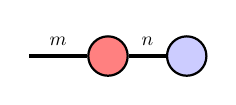
\begin{tikzpicture}[baseline=-0.5ex]
    \tikzset{tensor/.style = {minimum size = 0.5cm,shape = circle,thick,draw=black,inner sep = 0pt},
             edge/.style   = {thick,line width=.4mm},every loop/.style={}}
    \def\x{0}\def\y{0}
    \node[tensor,fill=red!50!white] (A) at (\x,\y){$\Ab$};
    \node[tensor,fill=blue!20!white] (x) at (\x+1,\y){$\xb$};
    \draw[edge] (A) -- (x) node [midway,above]{\scalebox{0.7}{\dimcolor{$n$}}};
    \draw[edge] (A) -- (\x-1,\y) node [midway,above]{\scalebox{0.7}{\dimcolor{$m$}}};
\end{tikzpicture}
\in\RR^{m}.
$$
线性是指对一切 $\alpha,\beta\in\RR$ 与 $\xb,\zb\in\RR^n$ 都有 $\Ab(\alpha \xb+\beta \zb)=\alpha \Ab\xb+\beta \Ab\zb$。当映射\emph{对每个自变量分别线性}时，张量便是其自然推广。具体地说，一个 $N$ 阶张量 $\Tt\in\RR^{d_1\times\cdots\times d_N}$ 定义了一个映射：它接受 $N$ 个输入向量，并沿所有模收缩而给出一个标量：
$$
f(\xb^{(1)},\dots,\xb^{(N)})
:= \langle \Tt,\ \xb^{(1)}\outprod \cdots \outprod \xb^{(N)}\rangle
=
\sum_{i_1=1}^{d_1}\cdots\sum_{i_N=1}^{d_N}\Tt_{i_1\cdots i_N}\,\xb^{(1)}_{i_1}\cdots \xb^{(N)}_{i_N}.
$$
该映射是\emph{多重线性}的：固定其余向量时，它对每个 $\xb^{(k)}$ 都是线性的。在张量网络图中，这就是
\[
f(\ab,\bb,\dots,\zb)
=
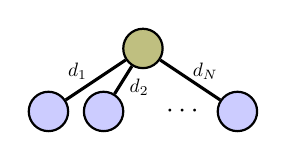
\begin{tikzpicture}[baseline=2ex]
    \tikzset{tensor/.style = {minimum size = 0.5cm,shape = circle,thick,draw=black,inner sep = 0pt},
             edge/.style   = {thick,line width=.4mm},
             every loop/.style={}}
    \def\x{0}\def\y{0}

    \node[tensor,fill=green!50!red!50!white] (T) at (\x,\y+0.8){$\Tt$};

    \node[tensor,fill=blue!20!white] (a) at (\x-1.2,\y){$\ab$};
    \node[tensor,fill=blue!20!white] (b) at (\x-0.5,\y){$\bb$};
    \node[draw=none] (dots) at (\x+0.5,\y){$\cdots$};
    \node[tensor,fill=blue!20!white] (z) at (\x+1.2,\y){$\zb$};

    \draw[edge] (T) -- (a) node [near end,above]{\scalebox{0.7}{\dimcolor{$d_1\ $}}};
    \draw[edge] (T) -- (b) node [near end,right]{\scalebox{0.7}{\dimcolor{$d_2$}}};
    \draw[edge] (T) -- (z) node [near end,above]{\scalebox{0.7}{\dimcolor{$d_N$}}};
\end{tikzpicture}
\in\RR,
\]
其中 $\ab, \bb,\cdots,\zb\in\RR^d$。
若留出一条腿不作收缩，便得到一个\emph{向量值}多重线性映射。例如，若 $\Tt\in\RR^{d_1\times\cdots\times d_N \times p}$，则除最后一个模之外对所有的模收缩，就定义了一个输出为 $p$ 维向量的多重线性映射：
$$
f(\ab,\bb,\dots,\zb)
=
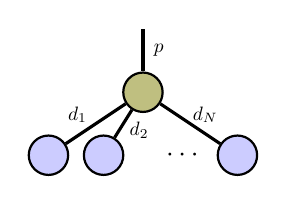
\begin{tikzpicture}[baseline=2ex]
    \tikzset{tensor/.style = {minimum size = 0.5cm,shape = circle,thick,draw=black,inner sep = 0pt},
             edge/.style   = {thick,line width=.4mm},
             every loop/.style={}}
    \def\x{0}\def\y{0}

    \node[tensor,fill=green!50!red!50!white] (T) at (\x,\y+0.8){$\Tt$};

    \node[tensor,fill=blue!20!white] (a) at (\x-1.2,\y){$\ab$};
    \node[tensor,fill=blue!20!white] (b) at (\x-0.5,\y){$\bb$};
    \node[draw=none] (dots) at (\x+0.5,\y){$\cdots$};
    \node[tensor,fill=blue!20!white] (z) at (\x+1.2,\y){$\zb$};

    \draw[edge] (T) -- (a) node [near end,above]{\scalebox{0.7}{\dimcolor{$d_1\ $}}};
    \draw[edge] (T) -- (b) node [near end,right]{\scalebox{0.7}{\dimcolor{$d_2$}}};
    \draw[edge] (T) -- (z) node [near end,above]{\scalebox{0.7}{\dimcolor{$d_N$}}};
    \draw[edge] (T) -- (\x,\y+1.6) node [midway,right]{\scalebox{0.7}{\dimcolor{$p$}}};
\end{tikzpicture}
\in\RR^p.
$$

